\documentclass[12pt]{report} 

% PACKAGES 
\usepackage[dutch]{babel}
\usepackage[utf8]{inputenc}
\usepackage{color}
\usepackage{amsmath} % Matrices
\usepackage{booktabs}
\usepackage{xcolor}
\usepackage{graphicx}
\usepackage{sectsty}
\usepackage{lipsum}
\usepackage{listings}
\usepackage[pageanchor=false]{hyperref} % hyperlinks in PDF


\partfont{\color{brown}}
\chapterfont{\color{teal}}
\sectionfont{\color{cyan}}

\lstset{language=C++,
                basicstyle=\ttfamily,
                keywordstyle=\color{blue}\ttfamily,
                stringstyle=\color{red}\ttfamily,
                commentstyle=\color{green}\ttfamily,
                morecomment=[l][\color{magenta}]{\#},
                frame = single,
                numbers=left,
	        stepnumber=1
}

% DOCUMENT INFORMATION
\title{Samenvatting Gegevensstructuren en Algoritmen}
\author{Bert De Saffel}
\date{2017-2018}


% CUSTOM COMMANDS
\setlength{\parindent}{0mm}
\setlength{\parskip}{1em}
\graphicspath{{./img/}}
\newcommand{\note}[1]{
  \color{violet}#1 \color{black}
}
\newcommand{\todo}[1] {
  \color{red}\textunderscore{\textit{TODO: #1}}
}

\def\lc{\left\lceil}   
\def\rc{\right\rceil}
\def\lf{\left\lfloor}   
\def\rf{\right\rfloor}


% DOCUMENT
\begin{document}
\maketitle
\tableofcontents

\part{Theorie}
\chapter{Inleiding}
Een algoritme is een verzameling van opeenvolgende instructies die uitgevoerd worden. Bij een het oplossen van een probleem zijn er twee zaken belangrijk:
\begin{itemize}
 \item De juiste aanpak gebruiken (Het algoritme).
 \item Een goede efficiëntie (De gegevensstructuren).
\end{itemize}
De focus van deze cursus ligt op de discrete wiskunde. Voor de continue wiskunde zijn er numerieke algoritmen nodig die niet behandeld worden in deze cursus.
\chapter{Efficëntie van algoritmen}
\section{Analyse van algoritmen}
\textbf{Probleem:} Er bestaat een vector $\note{v}$ met $\note{n}$ getallen. Er moet gezocht worden of er dubbele waarden in deze vector bestaan. Een eerste oplossing zou zijn:
\begin{lstlisting}
bool doubles = false;
 for(int i = 0; i < n; i++){
  for(int j = 0; j < n; j++){
    if(i != j && v[i] = v[j]{
      doubles = true;
    }
  }
}
\end{lstlisting}
Deze oplossing heeft volgende nadelen:
\begin{itemize}
 \item Indien er een dubbele waarde is gevonden, wordt er nog altijd verder gezocht.
 \item Als gevolg heeft dit dat de vector tweemaal wordt doorlopen.
 \item Het if statement op lijn 4 wordt uitgevoerd als bijvoorbeeld $i = 5$ en $j = 27$, maar ook als $i = 27$ en $j = 5$. Er is dus sprake van redundantie.
\end{itemize}
Een betere oplossing zou kunnen zijn:
\begin{lstlisting}
int i = 0;
int j = 1;
while(i < n && v[i] != v[j]){
  j++;
  if(j == n){
    i++;
    j = i + 1;
  }
}
\end{lstlisting}
De eerste keer wordt de while $\note{n}$ keer uitgevoerd, de tweede keer $\note{n - 1}$ keer tot uiteindelijk de while nog maar 1 keer uitgevoerd wordt. 


Het beste algoritme blijkt het volgende:
\begin{lstlisting}
vector<bool> zitErIn(n, false);
int i = 0;
while(i < n && !zitErIn[v[i]]){
  zitErIn[v[i]] = true;
  i++;
}
\end{lstlisting}
Het voordeel van bovenstaand algoritme is dat de while lus hoogstens $\note{n}$ keer uitgevoerd wordt.

\subsection{Tijdscomplexiteit}
Het is nuttig om te bekijken welke operaties een impact hebben op een algoritme. Beschouw volgende implementatie van het \textit{insertion sort} algoritme:

\begin{lstlisting}[escapechar=\%]
void insertion_sort(vector<T> & v){
  for(int %\fbox{\parbox{32pt}{i = 0}}%; %\fbox{\parbox{76pt}{i < v.size()}}% ; %\fbox{\parbox{26pt}{i ++}}%){
    %\fbox{\parbox{114pt}{T el = move(v[i]);}}%
    %\fbox{\parbox{90pt}{int j = i - 1;}}%
    while(%\fbox{\parbox{36pt}{j $\geq$ 0}}% && %\fbox{\parbox{64pt}{el < v[i]}}%){
      %\fbox{\parbox{140pt}{v[j + 1] = move(v[j]);}}%
      %\fbox{\parbox{26pt}{j--;}}%
    }
    %\fbox{\parbox{140pt}{v[j + 1] = move(el);}}%
  }
}
\end{lstlisting}
Elke relevante operatie werd omkaderd en heeft een bepaalde uitvoeringstijd $t$. Voor elke operatie kan de uitvoeringstijd apart beschouwd worden in zijn slechtste en beste geval:

\begin{tabular}{|l | l |l |l|}
  \hline
  Operatie          & Tijd  & Aantal(best) & Aantal(slechtst)  \\
  \hline
  h           & $t_1$ & 1            & 1                 \\
  i $<$ v.size()      & $t_2$ & n            & n                 \\
  i++               & $t_3$ & n - 1        & n - 1             \\
  T el = move(v[i]) & $t_4$ & n - 1        & n - 1             \\
  int j = i - 1     & $t_5$ & n - 1        & n - 1             \\
  j $\geq$ 0        & $t_6$ & n - 1        & (n + 2)(n - 1)/2  \\
  h < v[j]          & $t_7$ & n - 1        & n(n - 1)/2        \\
  v[j + 1] = v[j]   & $t_8$ & 0            & n(n - 1)/2        \\
  j--               & $t_9$ & 0            & n(n - 1)/2        \\
  v[j + 1]          & $t_10$ & n - 1            & n - 1)        \\
  \hline
\end{tabular}
\newline
\begin{itemize}
 \item Beste geval: $$(t_1 + t_8 + t_9) * 1 + (t_2 + t_3 + t_4 + t_5 + t_6 + t_7 + t_{10}) * n$$
Er kan ook gezegd worden dat de tijdscomplexiteit in het beste geval gelijk is aan $O(n)$
\item Slechtste geval: $$(t_1) * 1 + (t_2 + t_3 + t_4 + t_5 + t_{10}) * n + (t_6 + t_7 + t_8 + t_9) * n^2$$
Er kan ook gezegd worden dat de tijdscomplexiteit in het beste geval gelijk is aan $O(n^2)$
\end{itemize}
Het bewijs dat enkel de hoogste term de complexiteit bepaalt staat op pagina 10 van de cursus.
\section{Asymptotische benadering}
Een asymptotische benadering wil zeggen dat de uitvoeringstijd van een algoritme, vanaf voldoende grote waarden voor n, benadert kunnen worden met functies (Een begrenzende functie). Om deze begrenzende functie voor te stellen bestaan er drie notaties, namelijk: O, $\Theta$ en $\Omega$.
Onthou dat in de volgende voorbeelden de letter\note{n} het aantal elementen voorstelt.
\subsection{O-notatie}
De O-notatie stelt een afschatting naar boven voor. Dit wil zeggen dat een functie (het algoritme) niet sneller groeit dan een andere bepaalde functie, wat dus de bovengrens vormt. Zo wil de uitdrukking $O(n^2)$ zeggen dat het algoritme zeker niet sneller (maar wel gelijk) kan groeien dan de functie $n^2$. 
\subsection{Omega-notatie}
De $\Omega$-notatie stelt een afschatting naar onder voor. Dit wil zeggen dat een functie (ook weer het algoritme) niet trager groeit dan een andere bepaalde functie, wat de ondergrens vormt. Zo wil de uitdrukking $\Omega(n^2)$ zeggen dat het algoritme zeker niet traag (maar wel gelijk) kan groeien dan de functie $n^2$
\subsection{Theta-notatie}
Indien de ondergrens gelijk is aan de bovengrens wordt de $\Theta$-notatie gebruikt. 
\subsection{Voorbeeld: sorteren}
Indien een tabel met $n$ \textit{verschillende} elementen gegeven is, bestaan er $n!$ verschillende permutaties van $n$ elementen. Wat is het efficiëntste sorteeralgoritme? begin vanaf de ongelijkheid $n! < n^n$.

$$ n! < n^n$$ 
$$\log(n!) = O(n\log n)$$
$$\frac{n}{2}*(\frac{n}{2}+1) ... n$$
$$n! > (\frac{n}{2})^{n/2}$$
$$\log n! > \frac{n}{2}\log\frac{n}{2}$$
$$\log n! = \Theta(n\log n)$$
\section{Afschatten van recursiebetrekkingen}
Soms is het mogelijk een functie f af te schatten door een recursieve betrekking.
\subsection{Machten van n}
$$f(n) \leq Cn^{\alpha} + f(n - 1)$$
$$\leq Cn^\alpha + C(n - 1)^\alpha + f(n - 2)$$
$$\leq C(n^\alpha + (n - 1)^\alpha) + ... 1^\alpha) + f(0)$$
De term tussen haakjes kan geschreven worden als de integraal: 
$$n^\alpha + (n - 1)^\alpha) + ... 1^\alpha = \int_{0}^{n} \lc x\rc^\alpha dx$$
\subsection{Logaritmische afschattingen}
$$f(n) = f\bigg(\frac{n}{2}\bigg) + C$$
$$= f\bigg(\frac{n}{4}\bigg) + C + C$$
$$= f\bigg(\frac{n}{2^k}\bigg) + kC$$
indien k groot genoeg wordt
$$f(1) + kC\; \hbox{met}\; k = \lc\log n \rc$$
\subsection{Afschatting met sommen}
$$(x - 1)(1 + x + x^2 + ... + x^p)$$
$$= x + x^2 + x^3 + ... + x^{p + 1} - 1 - x - x^2 - ... - x^p$$
$$= - 1 + x^{p + 1}$$
Gevolg:
$$1 + x + ... + x^p = \frac{x^{p + 1}}{x-1} = S(x, p)$$
$$x^p < S(x, p) < x^{p + 1} \; \hbox{voor}\; x \geq 2$$
$$x + 2x^2 + 3x^3 + ... + px^p < px^{p + 1}$$
\subsection{Bernouilliverdeling}
Iets heeft een kans p om te mislukken.
$$p = \frac{1}{10e}$$
Een bepaald algoritme moet een slaagkans hebben van 80\%. Zal dit lukken met de kans p?
De kans dat er bij $m$ pogingen het $j$ keer misgaat is:
$$\sum_{k=0}^{k=j}C^{k}_{m}(1 - p)^{m-k}p^k < \sum_{k=0}^{k=j}\bigg(\frac{emp}{k}\bigg)^k$$
\section{Optimalisatie}
Stel een algoritme $a$ met 2 afschattingen.
$$
  \begin{cases}
    f_1(n) = \Omega(g_1(n)) \rightarrow \hbox{Actie}\; f_1(n)\; \hbox{keer}\\
    f_2(n) = \Omega(g_2(n)) \rightarrow \hbox{efficiëntie van 1 actie}\\
  \end{cases}
$$
De afschatting wordt $\Omega(g_1(n)g_2(n))$
Een voorbeeld is een quizwedstrijd. Bij een quiz mag elke ploeg een prijs kiezen, en dit in volgorde van de uitslag. Stel dat deze uitslag gegeven is in een tabel \texttt{uitslag} zodang dat \texttt{uitslag[i]} aangeeft wat de rangschikking is van ploeg \textit{i}. Er bestaan twee manieren om ploegen in volgorde aan te spreken.
\begin{lstlisting}
 for(int i = 0; i < n ; i++){
  int j = 0;
  while ( uitslag[j] != i){
    j++;
  }
  kies(j);
 }
\end{lstlisting}
De forlus ($g_1(n)$) wordt $n$ keer uitgevoerd. De whilelus ($g_2(n)$) wordt ook $n$ keer uitgevoerd. De afschatting wordt dus
$$\Omega(g_1(n)g_2(n)) = \Omega(n^2)$$
Een betere methode:
\begin{lstlisting}
 vector<int> invers(n);
 for(int i = 0; i < n; i++){
  invers[uitslag[i]] = i;
 }
 for(int j = 0; j < n; j++){
  kies[invers[j]);
 }
\end{lstlisting}
Dit voorbeeld heeft geen geneste lus, wat ervoor zorgt dat de afschatting $\Omega(n)$ wordt.
\chapter{Rangschikking}
Belangrijk bij sorteeralgoritmes:
\begin{itemize}
 \item Het aantal gegevens
 \item De aard van die gegevens
 \item De mate waarin de gegevens reeds geordend zijn
 \item De plaats waar de gegevens tijdens het rangschikken opgeslagen zijn (inwendig of uitwendig geheugen)
\end{itemize}

Er wordt aandacht besteedt aan drie zaken:
\begin{itemize}
 \item Tijdsefficiëntie
 \item Geheugengebruik
 \item Stabiliteit
\end{itemize}

Veronderstellingen:
\begin{itemize}
 \item Alle gegevens bevinden zich in het inwendig geheugen.
 \item De gegevens worden ondergebracht in een één dimensionale tabel.
 \item De gegevens zijn klein en bevatten geen bijhorende informatie.
 \item Er wordt gerangschikt in stijgende volgorde.
\end{itemize}

\section{Insertion Sort}
\begin{lstlisting}
void insertion_sort(vector<T> & v){
  for(int i = 0; i < v.size(); i++){
    T el = move(v[i]);
    int j = i - 1;
    while(j <= 0 && el < v[i]){
      v[j + 1] = move(v[j]);
      j--;
    }
    v[j + 1] = move(el);
  }
}
\end{lstlisting}
\subsection{Werking}
Insertion sort is een eenvoudig algoritme dat element per element werkt.
Vergelijk een element met de opeenvolgende elementen in de tabel. Schuif de grotere elementen op en zet het element op zijn plaats. De gerangschikte en nog te rangschikken zones hebben geen overlap.

\subsubsection{Slechtste geval}
Wanneer de tabel in omgekeerde volgorde gesorteerd staat. 
\subsubsection{Gemiddelde geval}

\subsubsection{Beste geval}
\subsection{Voordelen}
\subsection{Nadelen}
\textbf{straight from notities}

O(n + aantal inversies)

tabel v

vomgekeerd[i] = v[n - 1 - i];

vomgekeerd[n - 1 - i] > omgekeerd[n - 1 - j];

\# inversies in v + \#inversies in vomgekeerd = $\frac{n(n - 1)}{2}$



random tabel

\section{Shell Sort}

................


\section{Selection Sort}
.........

\chapter{Efficiënte Methodes}
\section{Heaps ( = Binaire boom)}
Een heap lijkt sterk op een gelinkte lijst, maar elke knoop heeft slechts 1 ouder en potentieël 2 kinderen. Een heap loopt van boven naar beneden. Het topelement wordt de \textit{wortel} genoemd. Een knoop zonder kinderen wordt een \textit{blad} genoemd. Een heap moet voldoen aan de \textit{heapvoorwaarde}: Elke sleutel van een knoop heeft een hogere prioriteit dan de sleutels van zijn kinderen.

Het verband tussen het aantal knopen $n$ en de hoogte $h$: $h = \lf \ln n \rf$

\subsection{Bewerkingen op heaps}
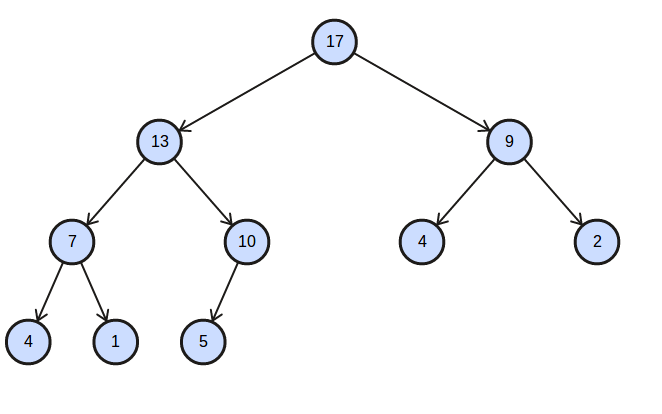
\includegraphics[width=\textwidth]{heap_1}
Toevoegen van een knoop (14)

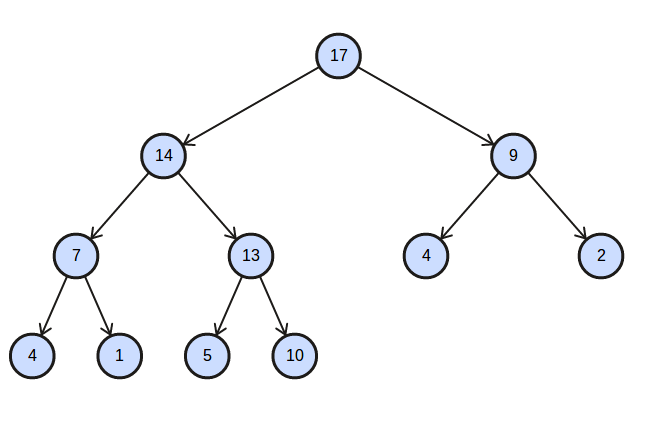
\includegraphics[width=\textwidth]{heap_2}
Het wortelelement vervangen(17 $\rightarrow$ 3)

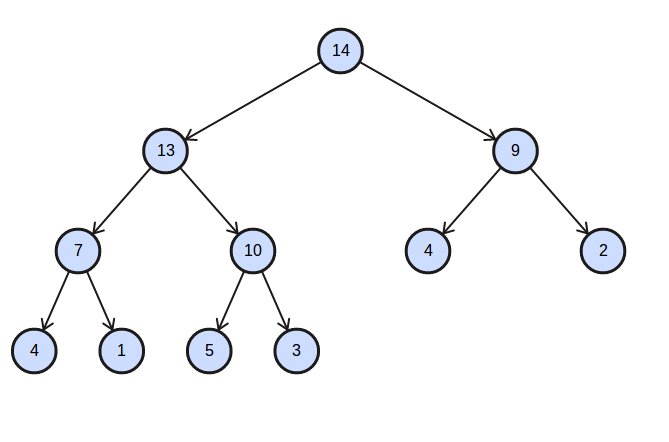
\includegraphics[width=\textwidth]{heap_3}
Het wortelelement verwijderen

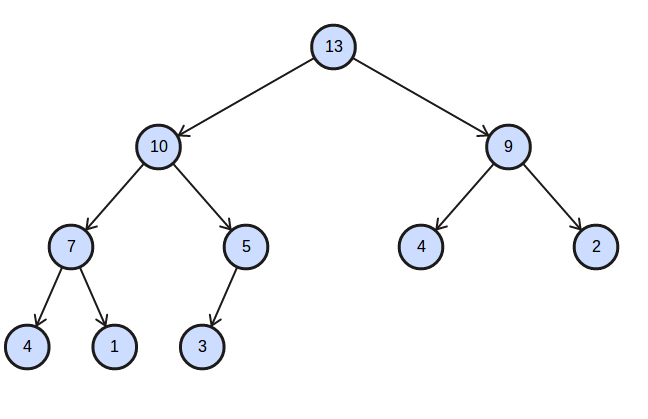
\includegraphics[width=\textwidth]{heap_4}

\subsection{Constructie van een heap}
Element toevoegen
Samenvoegen van deelheaps

\section{Heapsort}
\section{Mergesort}
\section{Quicksort}
\begin{lstlisting}
void quicksort (vector<T> & v, int l, int r){
    // rangschikt de deelvector v[l..r]
    if(l < r){
        //partitie met v[l] als spilelement
        T pivot = v[l]; // Geen T&, geen move!
        int i = l;
        int j = r;
        while(v[j] > pivot){
            j--;
        }
        while(i < j){
            swap(v[i], v[j]);
            i++;
            while(v[i] < pivot){
                i++;
            }
            j--;
            while(v[j] > pivot){
                j--;
            }
        }
        //Recursief rangschikken van beide delen
        quicksort(v, l, j);
        quicksort(v, j + 1, r);
    }
}

void quicksort (vector<T> & v){
    quicksort(v, 0, v.size());
}
\end{lstlisting}
\subsection{Werking}
Quicksort is een typisch voorbeeld van een Las Vegas algoritme. De originele tabel wordt opgepslitst in twee delen zodat alle elementen in het linkerdeel kleiner zijn dan de elementen in het rechterdeel.

Er wordt een willekeurige element (de pivot) gekozen. Er worden twee lijsten gemaakt met de ene lijst allemaal elementen kleiner dan de pivot en de andere lijst allemaal groter dan de pivot. Op deze deellijsten wordt er recursief ook quicksort toegepast totdat de grootte van de deellijst gelijk is aan 1.

Volgens de klassieke methode wordt het eerste element in de tabel gekozen als pivot.
Beschouw de volgende lijst:


\begin{tabular}{| c | c | c | c | c | c | c | c | c | c | c | c |}
 \hline
 10 & 10 & 3 & 9 & 17 & 2 & 9 & 8 & 10 & 16 & 15 & 4 \\
 \hline
\end{tabular}

Als pivot wordt het eerste element gekozen, dus 10. De variabele $i$ staat op index 0, de variabele $j$ staat op index 11 (laatste element). De waarde 4 is kleiner dan de waarde 10, dus deze worden omgewisseld.

\begin{tabular}{| c | c | c | c | c | c | c | c | c | c | c | c |}
 \hline
 4 & 10 & 3 & 9 & 17 & 2 & 9 & 8 & 10 & 16 & 15 & 10 \\
 \hline
\end{tabular}
\subsubsection{Slechtste geval}
\begin{equation*}
 \begin{split}
  T(n)          & = cn + T(n - 1)\\
                & = cn + c(n - 1) + T(n - 2) \\
                & = c(n + (n - 1) + (n - 2) + ... + 1) + T(1) \\
                & =c\frac{n(n - 1)}{2} \\
                & = O(n^2)
 \end{split}
\end{equation*}

\subsubsection{Gemiddeld geval}
Wanneer de pivot gemiddeld in het midden van de te partitioneren elementen valt. De grootte van elke deeltabel is dus even waarschijnlijk.
\begin{equation*}
 \begin{split}
  T(n) & = O(n \ln n)
 \end{split}
\end{equation*}
\subsubsection{Beste geval}
De beide delen zijn even groot.
$$T(n) = O(n \ln n)$$



\chapter{Speciale methodes}
\section{Ondergrens voor de efficiëntie van rangschikken}
Wat is de snelst mogelijke manier om te sorteren? De efficiënte methoden uit vorig hoofdstuk waren in het slechtste geval $O(n \log n)$ (behalve quicksort met $O(n^2)$). Er bestaan geen snellere methoden die een betere slechtste geval hebben. Dit wordt bewezen met een binaire boom.

Stel een beslissingsboom die vergelijkingen voorstelt. De eerste vergelijking bevindt zich aan de wortel van de boom. De tweede vergelijking in één van de kindknopen van de wortel enz... totdat het juiste resultaat gevonden wordt.

Voor elk sorteeralgoritme kan zo een boom opgesteld worden en zullen allemaal $n!$ bladeren hebben. Het aantal sleutelvergelijkingen dat een algoritme nodig heeft komt overeen met de lengte van de afgelegde weg. Zowel voor het slechtste geval als het gemiddelde geval is de ondergrens $\Omega(n \ln n)$.
\subsubsection{Slechtste geval}
\begin{itemize}
 \item Langst mogelijke weg van wortel naar blad = hoogte van de boom.
 \item Boom met hoogte h $\Rightarrow$ niet meer dan $2^h$.
 \item Boom met hoogte $h \Rightarrow$ twee deelbomen met hoogte $h - 1$
 \item $\Rightarrow 2^{h - 1} < n! \leq 2^h$ waaruit volgt $h = \lc \ln n! \rc$
 \item Met formule van Stirling blijkt $h > \ln (\frac{n}{e})^n$
 \item $\Rightarrow$ h = $\Omega(n \ln n)$
\end{itemize}
\subsubsection{Gemiddelde geval}
\begin{itemize}
 \item Gemiddelde weglengte van wortel naar blad
 
\end{itemize}

\section{Rangschikken door tellen}

\section{Radix Sort}



\end{document}
